\documentclass[a4paper,11pt,oneside]{article}

\usepackage[a4paper,top=3cm,bottom=3cm,left=3cm,right=3cm]{geometry}
\renewcommand{\familydefault}{\sfdefault}
\usepackage{helvet}
\usepackage{float}
\usepackage{parskip}
\usepackage{gensymb}
\usepackage[pdftex]{graphicx}
\usepackage[pdftex]{hyperref}
\pdfadjustspacing=1

\newcommand{\myname}{Dmitrii Cucleschin}
\newcommand{\mytitle}{Human-Machine Interaction Through Gesture Recognition (on the example of divers' sign language)}
\newcommand{\mysupervisor}{Prof. Andreas Birk}

\hypersetup{
  pdfauthor = {\myname},
  pdftitle = {\mytitle},
  pdfkeywords = {},
  colorlinks = {true},
  linkcolor = {blue}
}

\begin{document}
  \pagenumbering{roman}

  \thispagestyle{empty}

  \begin{flushright}
    
\includegraphics[scale=0.7]{bsc-logo}
  \end{flushright}
  \vspace{20mm}
  \begin{center}
    \huge
    \textbf{\mytitle}
  \end{center}
  \vspace*{4mm}
  \begin{center}
   \Large by
  \end{center}
  \vspace*{4mm}
  \begin{center}
    \Large
    \textbf{\myname}
  \end{center}
  \vspace*{20mm}
  \begin{center}
    \large
    Bachelor Thesis in Computer Science
  \end{center}
  \vfill
  \begin{flushright}
    \large
    \begin{tabular}{l}
      \mysupervisor \\
      \hline
      Name and title of the supervisor \\
      \\
    \end{tabular}
  \end{flushright}
  \vspace*{8mm}
  \begin{flushleft}
    \large
    Date of Submission: \today \\
    \rule{\textwidth}{1pt}
  \end{flushleft}
  \begin{center}
    \Large Jacobs University --- School of Engineering and Science
  \end{center}

  \newpage
  \thispagestyle{empty}

  With my signature, I certify that this thesis has been written by me
  using only the indicates resources and materials. Where I have
  presented data and results, the data and results are complete,
  genuine, and have been obtained by me unless otherwise acknowledged;
  where my results derive from computer programs, these computer
  programs have been written by me unless otherwise acknowledged. I
  further confirm that this thesis has not been submitted, either in
  part or as a whole, for any other academic degree at this or another
  institution.

  \vspace{20mm}

  Signature \hfill Place, Date

  \newpage

  \section*{Abstract.}
  
  Nowadays, we live in the world, where machines get more and more advanced and are tailored for a variety of different tasks. To initiate one of such tasks, person has to communicate the desired function to a machine through some sort of input device. Unfortunately, in some scenarios, common input devices (like keyboard and mouse) are unavailable and one has to implement a different communication method.\\
  \\
  In this thesis, I will be focusing on developing and testing one of such methods - communication with the machine via hand gestures. There are number of cases, where such method is more convenient than the analogues, but here we will focus on the specific case of integrating such a system in an underwater robot. Robot will be equipped with stereo camera and will be taught to recognize basic diver sign language. That will allow him to monitor health and safety of the human diver, as well as to receive instructions regarding the tasks and further steps it needs to perform from a distance. 

  \newpage
  \tableofcontents

  \clearpage
  \pagenumbering{arabic}

  \section{Introduction.}
  
  \subsection{Motivation.}
  
  Robotics department of Jacobs University Bremen has been working on several projects involving underwater robots. One of such projects, CADDY (Cognitive Autonomous Diving Buddy), is meant as an assistant for the diver, allowing to transport objects, take photographs and scan the surrounding area. However, equipment like this can be quite bulky and can possibly put the diver in danger in critical situations. Therefore, a concise communication method has to be implemented between human and robot to initiate tasks and report current danger status. Since CADDY is equipped with a depth camera, in this project we will be focusing on implementing one of such methods - communication using hand gestures. Equipped with an ability to recognize diver's sign language, CADDY will be able to be controlled from a safe distance, as well as to help diver and notify the others in case of any emergencies.
  
  \subsection{Research Question.}
  
  Based on the problem discussed above, the following research question arises, that I will be solving thorough my bachelor's thesis project:\\
  \textbf{Can a robust gesture-based communication system be implemented for a use in the underwater robot?}\\
  Since in a system like this reliability is very critical, it isn't enough to just implement the application logic. Thorough testing has to be performed to make sure all of the components of the system are functioning as expected. Therefore, the scope of this project isn't limited to research and implementation, but also quality assurance and creating proper design specifications.
  
  \subsection{Expected Research Contribution.}
  
  As a result of this research project, CADDY can be equipped with gesture recognition software, which will definitely be a very valuable addition to already impressive features of the device. With easy extensibility, it will be possible to extend the recognized gesture set and reuse this software in different projects. I feel that enabling people to communicate better and more naturally with the machine may simplify a lot of routine tasks, as well as potentially improve the speed of such communications, which may be crucial in the event of emergency situations.
  
%  \subsection{Outline.}
%  
%  This thesis paper briefly describes the steps that were taken to implement a basic version of diver's sign language recognition using a depth sensor (on an example of Kinect v2.0). The introduction presents the problem, as well as potential benefits of choosing this particular method. Next, state of the art section describes the overall progress and development in gesture recognition area, featuring some notable examples and experiments. Organizational issues, such as the project timeline, code license, deliverables and evaluation criteria are discussed. Final application, as well as bachelor's thesis will be developed according to specifications defined in this research proposal paper. 
  
  \section{State of the art.}
  
  Robot development has been advancing a lot over the course of last 10 years. We transcended all the way from simple programmable robots to truly autonomous machines, that can perceive the environment around them and interact with it. A lot of research has been done to perfect the communication with these "new-generation" robots. In 2006, a report \cite{SA01} has been published, that shows that natural interaction (speech recognition, face recognition, gesture processing, etc.) is a great way of performing such a task, because of variety of input data and emotional feedback as a result of such a communication. Furthermore, artificial intelligence researchers \cite{SA02} have discovered that when gesture recognition is present, humans tend to engage more with a robot and have better reviews, regarding their experience. However, such natural interfaces are not only useful for generic communication, but in some cases also for therapy. Robot AURORA \cite{SA03} aims to aid children with autism by being a salient observer with changeable behavior. Researchers note, that the emotional feedback is one of the most important variables in this scenario and natural interaction through speech and gestures help to achieve that.\\
  \\
  However, beyond research projects, the idea of implementing interface for consumer devices, controlled by natural interactions, isn't novel. At the moment, more and more manufacturers are investigating the possibility of adding voice or gesture control in their devices or applications. When the first Microsoft Kinect came out for Xbox 360, people were skeptical about the applications of a depth camera. Skeletal recognition and hand tracking were still quite choppy (partially due to hardware specifications and partially due to beta software) and controls using the camera were not intuitive and fluid. However, with the release of Xbox One and updated Kinect sensor, gesture control became one of the easiest ways to interact with the console. Kinect recognizes one of the three basic gestures: open hand, closed hand (fist) and lasso (2 fingers open), and bases interactions with the console on these. IR sensor with a better resolution allows for recognition in low- to no- light conditions. However, Microsoft isn't the only company, that is interested in providing such features. In their newest lineup of Smart TVs, Samsung introduced a feature \cite{SM01}, which allows basic control of your television with the gestures. Using a regular camera, that is built-in in the unit, TV can recognize simple gestures, like flip movement, thumbs up, selection etc. \\
  \\
  However, the potential of this technology isn't limited to just entertainment. Number of startups are working on the devices, which would allow developers to embed gesture control in any application (most notable examples are Leap Motion sensor and Myo armband). With the powerful SDKs, it's just a matter of time until the technology is perfected enough for gestural interaction to become an everyday part of our lives. There are already some impressive experiments using the power of gestures: Microsoft Research has presented a Kinect sign language translator for American and Chinese languages \cite{MS02}, as well as a tool for the hospitals that allows touchless interaction with the computer during surgeries \cite{MS03}.\\
  \\
  As we can see, even though the technology is still maturing and is not available to a lot of people, number of useful applications based on it is growing every day and the overall potential is very high.

 \section{Preparation.}

\subsection{Overview of Kinect 2.0.}

For the implementation of this project we will need a depth camera, that is able to produce a clear depth frame for the following hand segmentation and processing. While there are number of options to choose from, I chose \textbf{Microsoft Kinect 2.0}, because of its widespread availability and impressive specifications.\\

Second version of Kinect improved a lot over its predecessor, offering the following features:

\begin{itemize}
\item Color frames at 15-30 fps, depending on the light conditions (1920x1080)
\item Depth frames at 30 fps (512 x 424) with improved fidelity
\item Infrared frames at 30 fps (512 x 424)
\item Skeletal tracking of up to 6 users (25 joints per person)
\item Sound capture with an array of microphones
\end{itemize}

Kinect uses the following coordinate systems, that will be applied thorough the course of implementation of the project:

  \begin{figure}[H]
  \centering
  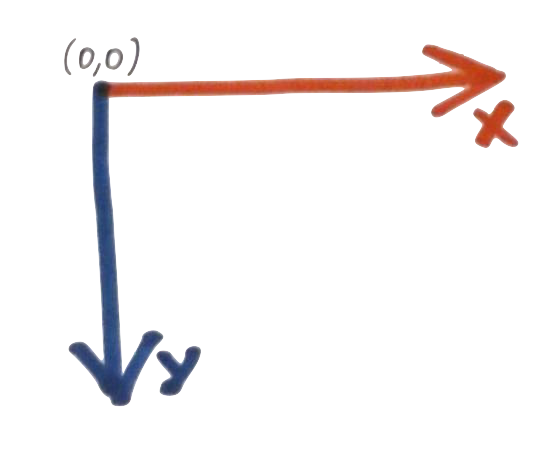
\includegraphics[scale=0.4]{coordinate-2d.png}
  \caption{Coordinate system for a 2D depth frame}
  \end{figure}

  \begin{figure}[H]
  \centering
  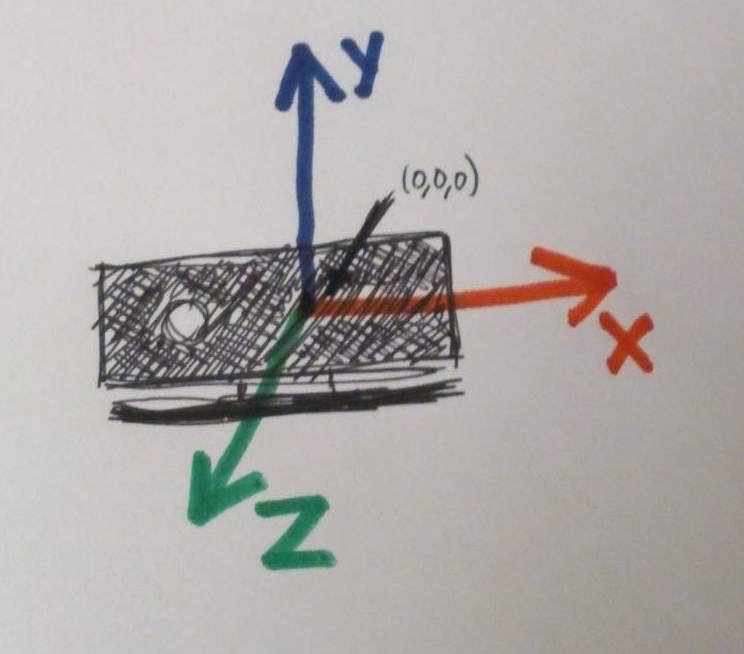
\includegraphics[scale=0.3]{coordinate-3d.png}
  \caption{Coordinate system for a 3D skeleton tracking frame}
  \end{figure}

\subsection{Choosing SDK.}

Microsoft has developed an \textbf{in-house SDK}, that is available as free download for every registered Windows/Kinect developer. It is used to take full advantage of all hardware capabilities of the sensor and includes a lot of helper utility functions, that ease the processing of the data. Drawback to using this approach is strict software limitation, allowing to only use it on Windows 8+ in the native C\# environment (wrappers for Java and other languages exist, but are not mature enough in their implementation to suffice for this project).\\

Alternative option is using \textbf{libfreenect2}, a UNIX library based on libusb, that allows basic interfacing with Kinect. The current version allows the export of raw unprocessed color, depth and IR data. It also requires basic reprogramming of Kinect sensor to bypass the software requirements and has no methods for matching frames to each other (converting points from one coordinate space to the other). Typically, as done with the first version of Kinect sensor, this data is later used with a generic processing library like \textbf{OpenNI} to calculate skeleton data and allow the use of other features. However, Kinect v2 is still on very early stages of support in OpenNI, not allowing the full skeletal tracking, needed for the scope of this application. Experiments also proved, that frame rate is far below fluent (average 3-5 fps), which is not suitable for this project.\\

As a result, we will base the implementation on native SDK, to allow us to unlock the full potential of the Kinect hardware, while allowing the fluid UI. We will also include \textbf{EmguCV}, a C\# wrapper of OpenCV to allow us to use otherwise complex algorithms, like Contours Detection, Convex Hull and Minimum Area Rotated Rectangle.
 
  \subsection{Gesture set}
	
    The following basic gesture set has been selected for the purposes of this project. Default semantics of those gestures are described, and the basic actions are assigned to them, based on some of the suggestions presented in CADDIAN language draft \cite{AB01}. Let's separate all the gestures into two kinds: \textbf{static}, corresponding to a single hand expression and \textbf{dynamic},  building upon the static ones, but also tracking hand animation (such as movement or a sequence of changing states). This list is meant only as the initial draft and should be easily extensible, once more features are needed.
    
    \subsubsection{Static gestures}
    
  \begin{figure}[H]
  \centering
  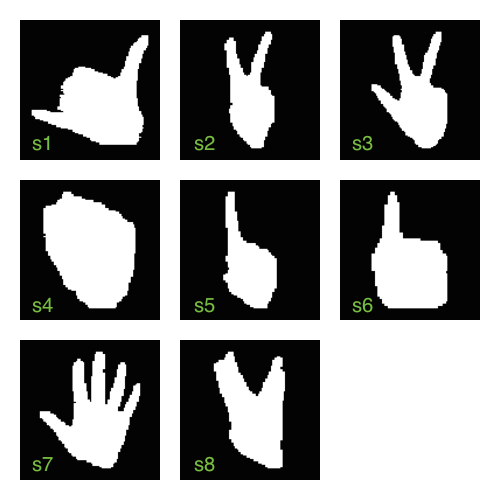
\includegraphics[scale=0.4]{static-gestureset.png}
  \caption{Static gesture set}
  \end{figure}
    
    \begin{itemize}
    \item \textbf{s1.} Ascend. The longer user keeps the gesture, bigger the priority.
    \item \textbf{s2.} Descend. The longer user keeps the gesture, bigger the priority.
    \item \textbf{s3.} Turn $90\degree$ to the right.
    \item \textbf{s4.} Turn $90\degree$ to the left.
    \item \textbf{s5.} Confirm action / Accelerate.
    \item \textbf{s6.} Cancel action / Decelerate.
    \item \textbf{s7.} Switch between piloting and task management (for gestures s6 and s7).
    \item \textbf{s8.} Predator (for example, shark) has been spotted, use caution.
    \item \textbf{s9.} Abort the current operation.
    \item \textbf{s10.} Contact the crew with operation logs and message from the diver.
    \item \textbf{s11.} Take a picture.
    \item \textbf{s12.} Take a picture and a 3D scan of surrounding area.
    \end{itemize}
    
    \subsubsection{Dynamic gestures}
    
  \begin{figure}[H]
  \centering
  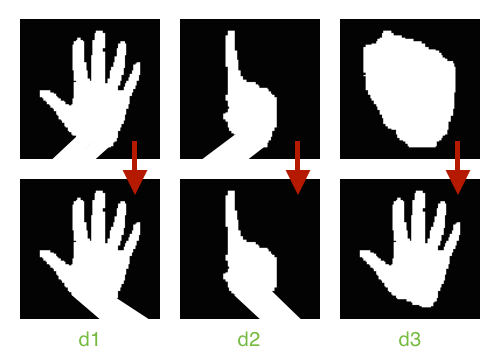
\includegraphics[scale=0.5]{dynamic-gestureset.png}
  \caption{Dynamic gesture set}
  \end{figure}
  
  \begin{itemize}
    \item \textbf{d1.} Emergency. Immediate abort of operations and ascend are requested. Faster the movement, bigger the priority.
    \item \textbf{d2.} Warning. Pause the operation and analyze the surroundings, contact the crew. Faster the movement, bigger the priority.
    \item \textbf{d3.} Closing and opening fist rapidly. Indicates that the oxygen is running out.
    \end{itemize}

\subsection{Environment assumptions.}

  For the purpose of this research project, the following assumptions will be made about the setup and the environment:\\
  
  \begin{itemize}
 \item Kinect is positioned to minimize the background noise (uncertain values).
  \item User is located directly in front of the sensor.
  \item View is not obstructed by any object in front of the user.
  \item There is only one user in the frame (multiple user tracking can be easily added, but adds computational intensity).
  \item When performing a gesture, hand is extended at least 30cm in front of the body.
\item Gesture recognition will be less robust in the scenario of a fast moving hand, due to the motion blur produced by the sensor
  \end{itemize}

\subsection{System requirements.}

As a result of choosing our depth camera and the SDK, the following system requirements need to be enforced to ensure the correct functionality of the application.

  \begin{itemize}
  \item 64-bit dual-core processor
  \item Dedicated USB 3.0 controller (Kinect will use its full capacity)
  \item $>$ 4 GB of RAM
  \item Graphics card with support of DirectX 11
  \item Windows 8 or newer
 \item Kinect v2 SDK and EmguCV installed
  \end{itemize}

  \subsection{Code License}
  
  All the code, written as the part of this research project will be available under \textbf{GPL v2} license. After the final submission, code will be available freely as an open-source repository hosted on Github. Anyone is free to use, modify or distribute this software and its parts, as long as they provide an attribution back and license it under the same terms.

 \section{Implementation.}

\subsection{Project structure.}

\begin{itemize}
\item \textbf{MainWindow}\\
Includes rendering of the main application window, initializing Kinect sensor and displaying the results of the recognition.

\item \textbf{FrameBuffer}\\
Stores last $n$ frames (in our case, 30) and provides easy access to interpolated frame data and gesture recognition results, that can be used to improve fluidity of the system and is needed for the dynamic gesture recognition.

\item \textbf{FrameProcessor}\\
Designed as a black box and is responsible for receiving the frame from Kinect, performing all the needed operations on it and storing it in the FrameBuffer. Event-based system is used, allowing to call MainWindow's delegate function to update the UI when needed, removing the necessity to wait for whole frame to process to get visual feedback.

\item \textbf{Utility}\\
Static class, including most global constants and helper functions, needed in the other classes.

\item \textbf{HandRecognizer}\\
Being initialized with an overall depth frame, this class is responsible for returning the segmented hand's binary mask, resized to a specific size for easier processing and comparison later on.

\item \textbf{Hand}\\
Processes the hand mask to locate and identify points of interest and other features to build a simplified model of a hand.

\item \textbf{Gesture}\\
Represents a configuration of the hand that corresponds to a defined gesture.

\item \textbf{GestureRecognizer}\\
Analyzes the model of the hand against a set of defined gestures to return possible matches.

\end{itemize}

\subsection{Capturing the frames.}

After the Kinect sensor is initialized, a reader is created to retrieve multi-source frames.  Since the robot will be submerged underwater, some frame sources become less effective for our implementation. For example, color frames will be very dark, where silhouette and background are almost indistinguishable and infrared frames will be distorted due to different propagation speed of the IR rays. Therefore, we will be capturing depth frames (which Kinect implements using measuring response time of laser beams) and skeleton tracking data, based on them. Another advantage of such an approach is an opportunity to swap Kinect for any other compatible device. Given any device to capture depth (could be a sonar or calibrated stereo camera) and a framework to track body joints (OpenNI, for example, is adaptable to almost any device), the following implementation can be adapted to work in these conditions with little changes to the main algorithms.\\

  \begin{figure}[H]
  \centering
  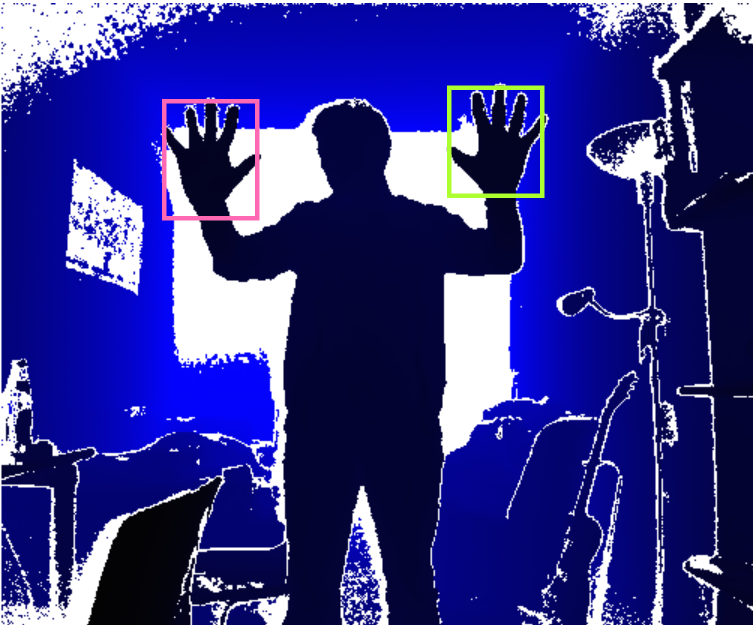
\includegraphics[scale=0.70]{depth-frame.png}
\caption{Depth frame returned by Kinect}
\end{figure}

After the frames are captured, the raw depth data in retrieved as \textit{ushort[]} with distances in millimeters to every pixels of a frame, ranging from 0 to 8000. Those values will be filtered to only make use of reliable values returned by sensor, which usually are within the range of 500 - 4500. After that, the body joints returned by the body frame will be synchronized to depth frame's 2D coordinate space, using the provided \textit{Kinect.CoordinateMapper} class.

  \subsection{Hand segmentation}
  
As a next step, we will analyze a pixel neighborhood, corresponding to hand joints, returned by the sensor. If those pixels are not a part of the body (in the other words, are in the background), we can judge that Kinect didn't return the right values for this frame and, therefore, can skip all the further processing. In the other case, a modified Scanline FloodFill algorithm will be used to segment and draw the binary mask of the hand. This particular version of algorithm was chosen for its superior efficiency, analyzing the lines of an image as opposed to individual pixels, resulting in much smaller queue size and thus, less iterations.\\

Instead of using a generic threshold in both directions, two separate thresholds will be used: one large one to apply to values closer than the hand's center (to ensure capturing of all the possible hand positions) and a smaller one to analyze values further away. That can be used only based on our previous assumption, that the hand is the closest object in sensor, allowing us to assume that no objects will interfere with forward thresholding. Additional check is implemented to check the distance from the hand's Z coordinate to the corresponding shoulder's Z coordinate (or head, if not available), that is aimed to minimize the number of cases, where the backwards threshold is large enough to segment bigger regions of the body, returning the data not suitable for proper gesture recognition.\\

In the algorithm, which detailed in the \textit{Appendix} section, additional check (denoted with \textit{BeyondWrist}) is made to crop values behind the wrist line. That is performed by disregarding all the pixels, projections of which on the plane, described by $v = (handX - wristX, handY - wristY)$, as returned by the Kinect sensor, are below the wrist point. However, due to noise in processing such a small region, often mistakes occur where the wrist point jumps and some fingers are being mistakenly cropped. That's why the current implementation doesn't rely on this and instead attempts to achieve different means of classifying the wrist region later on. Should a special identifying marker be allowed or additional calibration of Kinect  to return more precise coordinates, this method would return a very accurate representation of the wrist line.\\

  \begin{figure}[H]
  \centering
  
\includegraphics[scale=1.5]{hand-mask.png}
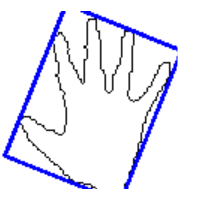
\includegraphics[scale=1.5]{hand-box.png}
\caption{Hand mask, its contour and minimum area rectangle}
\end{figure}

Resulting region then will be resized to a constant size (defined as 120x120 in my implementation) to remove variance based on hand's size and orientation of the sides of the bounding box (as suggested by \cite{HI01}).

  \subsection{Palm segmentation}
  
 Before identifying points of interest on our segmented binary image, let's consider which degrees of freedom does the hand allow. On the image below (taken from \cite{OT01}), we can see the general model of hand, as well as all its 26 degrees of freedom. While this model is mostly accurate, there are some people who might anatomically have an extra degree of freedom in their thumb. We will not consider such cases and instead focus on simplified version of the general model with bending angles achievable for an average person.\\
  
  \begin{figure}[H]
  \centering
  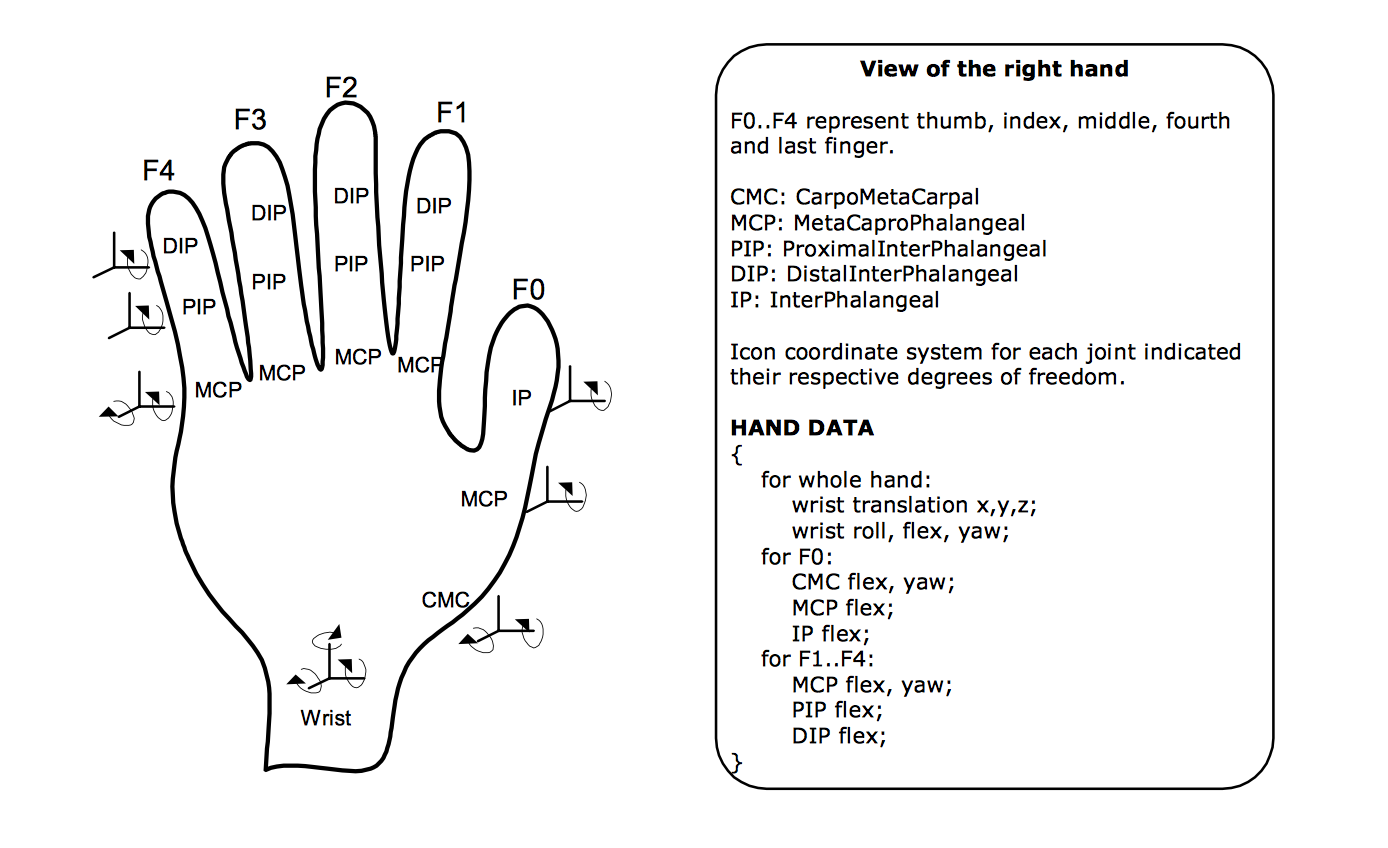
\includegraphics[scale=0.47]{hand-dof.png}
\caption{General model of the hand}
\end{figure}

Next step is to locate so-called "palm point", the center point of the palm, which will help us to identify the palm, segment it and determine approximate orientation of the hand. To do that, we will use an optimized 2D distance transform algorithm (as derived by \cite{DT01}), where the matrix of the same size as the mask is filled with distances to the closest pixel boundary. The point with $d[i] = max(d)$ (or an average if multiple points of this kind exist) is defined to be a palm point.\\

 Now, let's draw a circle around this point, increasing radius every time until non-skin values appear. Such a circle with a maximal radius will encompass the entire palm and is called inner circle. Once we've determined that, we can draw another circle, with the radius larger than inner circle's. Experimental factor of 1.5 was selected to separate the fingers, but retain the thumb even at its larger angle. This larger circle will function as a great mask, allowing us to analyze pixels outside of it for potential finger candidates.\\

The result of palm segmentation is illustrated at the image below:\\

  \begin{figure}[H]
  \centering
  
\includegraphics[scale=1.5]{hand-circles.png}
\caption{Palm center, inner and outer circles on the hand contour}
\end{figure}


\subsection{Finger recognition}

To find the regions, corresponding to fingers, we will sample the values (360 for the best precision), located on the larger circle. If the pixel belongs to the hand of the mask, a connected region will be analyzed using a simplified version of Flood Fill to yield a region, occupied by the finger. At this point, regions smaller than the specified area cutoff (defined experimentally to be 20 pixels), will be discarded as noise to avoid detecting extra fingers. It's possible then to traverse presumed finger regions to find a fingertip (which is anatomically defined to be the point, furthest away for the center of the palm), as well as directional vector pointing from the base to that point (representing a simplified model of a finger).\\

 \begin{figure}[H]
  \centering
  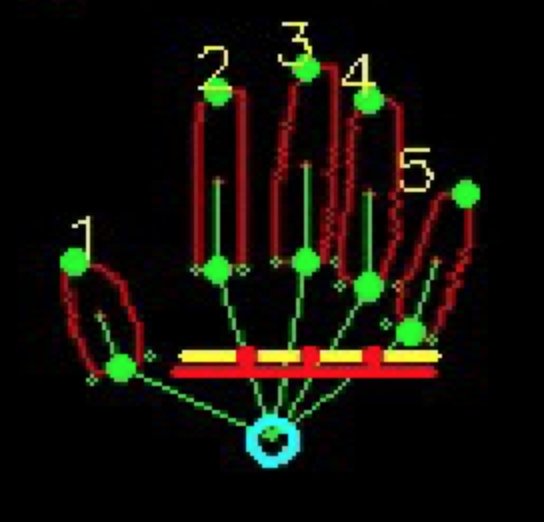
\includegraphics[scale=0.7]{hand-recognized.png}
  \caption{Model after finger recognition}
  \end{figure}

However, in some of the cases this will not be enough to make a correct judgement of a finger. If fingers are grouped together (located very close to each other), one bigger region will be returned, encompassing multiple fingers. In that case, rotated minimum area rectangle will be analyzed to make a prediction about a number of fingers inside the region. Let's define base width of that rectangle to be a length of a side, completely bordering with the outer circle of the hand. Now we can compare that value with a radius of the inner hand circle (representing the width of a segmented palm), decreased by 10\%, making it roughly the same as the width of 4 connected fingers. This computation will yield the following ratio (denoted $\lambda$):

\[\lambda = \frac{BaseWidth * 4}{InnerCircleRadius * 0.9} \]

The values of this ratio can be analyzed, using the robust constants as suggested by Vitali Henne \cite{VH01} to make the final approximation regarding the number of fingers in the region.

\begin{itemize}
\item $\lambda < 1.4$ : 1 finger in the region
\item $1.4 <= \lambda < 2.4$ : 2 fingers in the region
\item $2.4 <= \lambda < 3.4$ : 3 fingers in the region
\item $3.4 <= \lambda < 4.4$ : 4 fingers in the region
\item $\lambda >= 4.4$: Discard the case as anatomically impossible.
\end{itemize}
 
\subsection{Recognizing static gestures}
  
Now that we can build a simplified model of the hand, we can try to compare the hand to the set of predefined gestures to return the closest match. All the gestures are stored as JPEG files in \textit{Gestures} directory, representing the mask of the hand. When initialized, an additional argument is passed to the constructor, which is the number of fingers displayed (to avoid further computations).

Then, for every recognized model of the hand, the following methods are used to determine whether it represents a gesture:\\

\begin{itemize}
\item \textbf{Number of fingers comparison.}\\
Obviously, if the number of fingers on the hand doesn't match the desired one for the particular gesture, we should halt the computation immediately and jump to the next gesture. This check ensures that fewer contours are being analyzed and compared and allows us to increase the cutoff constants for the next two methods to allow more variation in the overall hand shape.\\

\item \textbf{Contour match.}\\
As a first step, we extract the contours from both the gesture image and original hand's mask image. Then, we can use the following formula to return the similarity between two contours:
\[ I(A,B) = max_{i=1..7} \frac{|m_i^A - m_i^B|}{|m_i^A|} \]
\[  m_i^A = sign_i^A * log (h_i^A) \]
\[  m_i^B = sign_i^B * log (h_i^B )\]

Here, $h_i^A$ and $h_i^B$ represent Hu moments of an image. Since the specific properties of Hu moments are rotation and scale invariance, this will allow us to detect gestures even when the hand is rotated.

It's important to note, however, that since we're detecting gestures in 2D space of a depth frame, rather than 3D space, some gestures may stop being recognized if the overall contour changes too much due to different perspective of a hand for the camera.  If the environment assumptions are fulfilled and hand is fully extended in front of the body, these problems will not arise.

After analyzing the output of the algorithm, a cutoff threshold for similarity was chosen to be 0.80.\\

\item \textbf{Histogram match.}\\
Since contour of the hand can be quite similar for different gestures, it's not enough to reliably determine whether a particular gesture has been shown. To solve this problem we will need to find another comparison metric, that would add confidence to our recognized gesture.

One of such metrics can be derived by calculating and comparing the 2D pair-wise geometrical histograms (PGH) of the images. The algorithm will calculate the angle and minimum/maximum distances for every pair of edges in the contour. This is done by selecting each of the edges as a base, while the function is looping through all other edges, recording distances from the points on the non-base edge and line of the base edge. The angle will define a row of the histogram in which all the bins that represent the distance between retrieved minimum and maximum distances are incremented.

The results are then normalized, to prevent the errors in the situation when two images are not of the same size. Finally two resulting PGHs are compared using Bhattacharyya distance, that is commonly used to measure similarity between two probability distributions:
\[ d(H_1, H_2) = \sqrt{1- \frac{1}{ \sqrt{H_1^{-} H_2^{-} N^2}}  \sum\limits_{I} \sqrt{H_1(I) H_2(I)}} \] 

After analyzing the output of the algorithm, a cutoff threshold for similarity was chosen to be 0.20.\\

\end{itemize}

In addition, another small threshold value is used for the product of the results of contour match and histogram match (cutoff threshold = 0.01). That ensures, that even if one of the values fluctuates, the overall similarity factor is very high.

Using this comparison method, the hand will be evaluated against the entire gesture set and the closest match satisfying the cutoff constraints will be returned.

In some of the cases (like \textbf{s1/s2} and \textbf{s5/s6}), the direction vector will be determined with regards to the inner circle, to determine which direction is the finger pointing to and choose the respective action. Additionally, since both hands are being tracked at the same time, more complex gestures can be defined using the combination of two hands (here, \textbf{s9}).

Since the algorithm relies heavily on shape and contour of the hand, it is possible that recognition results and precision may vary from a person to person. However, because of this nature of storing gestures as pictures, it's trivial to adapt the system to a particular user's hand to improve the reliability of the recognition algorithm. To do that, user has to show a desired gesture, press the "Save" button, and replace the existing gesture image (or add the new one) with the one outputted to the directory, from which the program is launched. 

//pichere\\\\

\subsection{Recognizing dynamic gestures}
  
Since dynamic gestures are happening across multiple frames, simple frame-by-frame analysis (as used for static gesture recognition) is not enough. Instead, we will retrieve the latest $n$ frames, stored in the frame buffer and analyze whether their features correspond to requirements set by the gesture. Here are some of the features, that we are interested in:

\begin{itemize}
\item Depth data of the frame.
\item Position and relative offset of the joints.
\item Position of hand's bounding box.
\item Number of fingers shown.
\item Static gesture(s) recognized.
\end{itemize}
 
For example, for gestures \textbf{d1} and \textbf{d2} we will analyze the last 30 frames (corresponding to roughly 1 second). Since the static gesture can not be successfully recognized in some cases due to motion blur, we will not impose strict requirements for all frames to match the required gesture. Instead, let's say that if gesture has been recognized in more than 80\% of frames, it will count as a successful recognition. Additionally, we track relative positions of elbow and hand joints, allowing us to build a simple state machine logic. We are starting in a neutral resting state, then we track displacement to the left and to the right. If it follows the "wave" pattern (movement to the left then to the right), the corresponding gesture is recognized.

In a case of \textbf{d3}, we can only the static gestures recognized. If we can notice the trend of rapid change from open hand to closed fist across the analyzed frames, we can judge that this gesture has been displayed. 

\section{Final deliverable.}
 
 \section{Evaluation.}
  
 Evaluation criteria for this research project are strongly coupled with the project requirements and implementation quality. The project is assessed against the following criteria, that can be used to evaluate the results of this thesis:

  \begin{itemize}
  \item \textbf{Functionality.} \\
Application successfully detects the fingers, displayed in a frame, invariant of the hand rotation and the presence of multiple fingers in the region. Furthermore, a basic classification is applied that aims to detect the thumb, among the fingers, to correctly continue with identification. However, due to the extreme noise in the data, provided by the Kinect sensor, the reliability of this is yet to be improved (by finding a reliable vector that can be used as a basis for angle calculation). Therefore, gesture recognition works only in the "perfect" cases and will be improved to be completely robust in the following research.

  \item \textbf{Correctness.} \\
10 test subjects of different gender and varying hand features were asked to use the application to analyze it for correctness. Experiment produced the following results:\\

\begin{itemize}
\item Hand is being correctly segmented in 100\% of the applicable cases.
\item Hand is being correctly ignored, based on all of the conditions (frontmost object in the frame, far enough from the body). The only case, that failed for 4 out of 10 participants, was the one, where user would be standing sideways (which is not a defined use case for our application). Then, shoulder Z coordinate would not be a reliable reference anymore, causing a bigger region (the entire arm) to be segmented. This can be improved by analyzing more joint values to detect the incorrect position of user with respect to the sensor.
\item Fingers were correctly located in 100\% of the cases, where hand was positioned normally (even when there were multiple fingers within a region). After testing with variant hand orientations, the success rate slightly drops to 70\%, based on accurateness of Kinect joint data.  A better wrist approximation would allow to immediately fix all of this cases, detecting the hand in every situation.
\item Static gestures were correctly recognized only in those cases, where hand was positioned perfectly and Kinect located the thumb point successfully, which results to about 5-10\% success rate. Once we will achieve the complete invariance, that was described above, expected success rate is 80-85\%, based on the inaccuracies in Kinect data and hardly recognizable (distorted) hand positions.
\item Dynamic gestures were not implemented yet, since all the work has been focused on improving the results of the previous steps. However, sampling points from various Kinect joints proved the correctness of the proposed algorithm in 95\% of test cases for every participant.
\end{itemize}

\item \textbf{Modularity.} \\
Adding new gestures to the application is trivially simple. A new Gesture object is created, describing the set of features needed to recognize the gesture and the desired callback. This object is later added to an array, maintained by GestureRecognizer to immediately enable it for processing. \\
Similar approach is used with dynamic gestures, except the additional step, which is overwriting the \textit{Evaluate()} function, that will implement the basic state machine and monitor the position of the hand across successive frames.

  \item \textbf{Code Quality and Documentation.} \\
Class structure presented above proves a very efficient way of separating this application, where each class has its own distinctive purpose and scope. Variables and methods have descriptive names, and overall C\# code design guidelines were enforced (checked using JetBrains' plugin, called Resharper).\\
Writing proper documentation is still a work-in-progress, but on the moment of final submission, there will be a complete generated HTML documentation included, describing every method, class variables and class completely (similar to Doxygen style). Furthermore, all details of the algorithms which were not intuitive have a short descriptions next to them, allowing people who build on top of this code to easily understand and tweak the working mechanics of this application.

  \item \textbf{Testing.}\\ 
Over the course of development I was adhering to \textbf{test-driven development} to minimize the time spent on fixing bugs and narrowing the source of potential problems. Small unit tester was written for every component of the application to assess the result of the operations we are relying on (for example, initializing the Kinect sensor) and implemented complex algorithms (like DT and FloodFill). That allowed me to be confident in the algorithms' correctness and instead focus on filtering the noise in sensor's measurements and input data. All the actual results were tested using a live demo to account for environment noise (application works perfectly when seeded with correct hand masks). 

  \end{itemize}

\section{Discussion.}

\subsection{Improving the results.}
Given the precise skeletal tracking, which sadly is not completely reliable with the Kinect SDK, much better approximation of the wrist line and location of the fingers can be made, skipping a lot of computation that we are doing to calculate the trusted points. Furthermore, if a state of a thumb is returned, we can make immediate assumptions about the state of the hand, again, simplifying the recognition a lot.

\subsection{Extending the application for more complex cases.}
Depth mask of the hand can be reused to calculate the differences in depth at midpoints and towards the fingertip to yield a better approximation of the general model of the hand. That will allow to define more features to describe the gesture and thus, expand the recognition far beyond the simple gesture set. Multiple sources familiar with gesture recognition recommend using Hidden Markov Models for such cases to define a machine learning algorithm that automatically gathers a set of relevant features from all of the available data. Application could then be extended to include a "learning mode", where user can add a new gesture to the set of available ones simply by training the algorithm on the number of applicable cases under different environment conditions.
  
 \section{Conclusion.}

 Summarizing all the information presented above, we can see that gesture recognition, despite being a pretty novel technology, has a lot of useful applications. In our case, communicating with robot underwater can be complicated due to a number of natural events. Gesture recognition system allows to control the robot from the safe distance and keep track of health conditions of the diver. Step-by-step implementation of gesture recognition was presented, starting from hand segmentation and ending with identifying different kinds of gestures. It proved quite reliable in specific cases and further work is being done to improve to be as robust as possible.  

  \section{Acknowledgements.}
I would like to thank all the people, who helped me to succeed with implementing this guided research project:

\begin{itemize}
\item My guided research instructor, Prof. Andreas Birk for the advice and assistance in the course of working on this thesis.
\item Prof. Horst Hahn for his excellent course in image processing, that I attended.
\item Alexandru Barbarosie for the invaluable advice in geometrical analysis of the hand features and filtering the noisy data out. 
\item Microsoft for providing me with Kinect v2 sensor to keep after my internship. 
\item Finally, there is no way I would reach where I am now without my family and friends - I thank them for their support and for making me the person, that I am today.
\end{itemize}

 \newpage

\section{Appendix}

\subsection{FloodFill implementation}

\begin{verbatim}
FloodFillCheck (x, y, startDepth, mask) : bool
     if (!IsValidPoint(x, y)) return false
     if (depth[x, y] is not reliable) return false
     if (mask[x, y] is already marked) return false
     if (depth[x, y] > startDepth + bwdThreshold) return false
     if (depth[x, y] < startDepth - fwdThreshold) return false
     // if (BeyondWrist(x, y) return false (!)
     return true

FloodFill (startPoint, startDepth) : Hand
     Queue q, Bool[] mask
     minX = minY = +Infinity
     maxX =  maxY = -Infinity

     mask[startPoint.X, startPoint.Y] = true
     q.Add(startPoint)

     while (q is not empty)
          p = q.Pop()

          w = p.X, e = p.X
          while (FloodFillCheck(w-1, y, startDepth, mask)
              w = w-1
              mask[w, p.Y] = true
              if (w < minX) minX = w
          while (FloodFillCheck(e+1, y, startDepth, mask)
              e = e+1
              mask[e, p.Y] = true
              if (e > maxX) maxX = e

         for (i in range (w, e)) 
              if (FloodFillCheck(i, y-1, startDepth, mask)
                  if (y-1 < minY) minY = y-1
                  q.Push(i, y-1)
              if (FloodFillCheck(i, y+1, startDepth, mask)
                  if (y+1 > maxY) maxY = y+1
                  q.Push(i, y+1)
     
     position = Rectangle(minX, minY, maxX - minX, maxY - minY)
     return Hand(position, mask)

\end{verbatim}

  \renewcommand{\refname}{\section{References}}
  
  \bibliographystyle{unsrt}
  \bibliography{thesis}

\end{document}